\documentclass[]{beamer}
\usepackage[T1]{fontenc}
\usepackage[utf8]{inputenc}
\usepackage[english]{babel}
\usepackage[babel]{csquotes}
% Graphics related packages:
\usepackage{tikz,pgfplots,graphicx,siunitx}
\DeclareSIUnit\torr{torr}
\usepackage[mode=buildnew]{standalone}
\usepackage{tikzscale}
\usepackage{ifthen} % used in fiber.tikz
\usetikzlibrary{calc} % used in fiber.tikz
\usetikzlibrary{math} % used in starkBroadening.tikz

%% To reduce compilation time
%\usepgfplotslibrary{external}
%\tikzexternalize

\usepackage{adjustbox} % for \adjincludegraphics for begin{columns}
%Information to be included in the title page:
% For tables:
\title{Low jitter plasma channel in 3D printed gas filled capillary discharges}
\subtitle{Thesis Presentation}
\author{Ehud Behar}
\institute{Hebrew University of Jerusalem}
\date{2021}

\AtBeginSection[]
{
  \begin{frame}
    \frametitle{Table of Contents}
    \tableofcontents[currentsection]
  \end{frame}
} % put the table of contents at the beginning of each section and highlight the title of the current section

% from https://tex.stackexchange.com/a/415653/180429
\setbeamertemplate{frametitle continuation}{\insertcontinuationcount}
\begin{document}

\frame{\titlepage}
\begin{frame}
\frametitle{Table of Contents}
\tableofcontents
\end{frame}

\section{Background}
\subsection{Theoretical Introduction}
  \begin{frame}{Linear accelerators}
  \begin{center}
    The goal is to design a table--top particle accelerator.
  \end{center}
  \end{frame}
  \begin{frame}{Linear accelerators}
    At present, all high energy accelerators run into limits.
    Requiring larger physical size and,

    The acclerating electric fields must be less than \SI{100}{\mega \V}, to avoid material breakdown.

    Each \si{\giga \eV} of energy requires $\sim$\SI{100}{\meter} of accleration length.
    \begin{figure}
      \includegraphics[width=200pt]{figures/theory/lhc_cern_compressed.jpg}
    \end{figure}
  \end{frame}
  \begin{frame}{LWFA}
  The idea: to build a plasma--based chraged particles accelerator.

  An intense short laser pulse generating a plasma wave wake as it propagates through the plasma.

  Electron trapped in the plasma wave can gain significant energy from the electric field of the plasma.
  \begin{figure}
    \includegraphics[width=300pt]{figures/theory/lwfa-schematic.PNG}
  \end{figure}
  \end{frame}
\newcommand{\whatisplasma}{What plasma is?}
\begin{frame}{Background to Electron acceleration}{Linear accelerators}
Plasma is defined as an ionized gas of charged and neutral particles, which  satisfies  the quasi–-neutrality condition.
\begin{figure}
    \centering
    %\includegraphics[width=0.5\textwidth]{figures/theory/temp_and_states.png}
\end{figure}
Molecules in the gas dissociate to form a gas of freely moving charged particles --- electrons and positive ions.
\end{frame}
\begin{frame}{\whatisplasma}
So, Plasma is a mixture of electrons, ions, and neutral particles moving in random directions that on the average is electrically neutral ($n_e \simeq n_i$).

In addition, plasmas are electrically conducting due to the presence of these free charge carriers and can attain electrical conductivities larger than metals such as gold and copper.
\end{frame}
\begin{frame}{Plasma characteristics}
It is customary to classify a plasma in terms of its electron temperature (measured in \si{\eV}) and electron densities (in \si{\per\cubic\cm}).
\vskip 1em
\begin{columns}
\column{0.5\textwidth}
One electron volt is equal to approximately \SI{11600}{\K}.
\column{0.5\textwidth}
Electron densities in the range \SIrange{e6}{e18}{\per\cubic\cm}
\end{columns}
\end{frame}
\newcommand{\debye}{Debye shielding length}
\begin{frame}{\debye}
  Debye length, $\lambda_D$, determines the effective interaction between charged particles in a plasma.
  \begin{equation*}
\lambda_D=\sqrt{\frac{\varepsilon_0 k_B T_e}{N_e e^2}}=\sqrt{\frac{k_B T}{m_e}}\frac{1}{\omega_p}.
\end{equation*}
\begin{itemize}
  \item Determined by the density and temperature of the plasma.
\end{itemize}
For a plasma with $T\approx \SI{1}{\eV}$ and $N_e\approx \SI{e18}{\per\cubic\cm}$, $\lambda_D\sim \SI{7}{\nm}$.

For any volume with a length scale $L$ satisfying 
\begin{equation*}
L \gg \lambda_D,
\label{eq:quasiNeutrality}
\end{equation*}
overall quasi-neutrality is a good approximation.
\end{frame}
\newcommand{\plasmafreq}{Plasma Frequency}
\begin{frame}{\plasmafreq}
This is the typical electrostatic oscillation frequency of electrons in response to a small charge separation.
\begin{figure}
  \includegraphics[width=100px]{figures/plasma_oscillation.PNG}
\end{figure}
\begin{equation*}
		\omega_p=\sqrt{\frac{N_e e^2}{m_e \varepsilon_0}}\si[per-mode=fraction]{\radian\per\sec}.\label{eq:plasma-frequency}
\end{equation*}
For a typical plasma density of $N_e \sim \SI{e18}{\per\cubic\cm}$, we get $\omega_p=\SI{5.6e13}{\radian\per\sec}$.%, which lies in the microwave range.
\end{frame}
\begin{frame}{The plasma parameter}
The plasma parameter $\Lambda$ is defined as
\begin{equation*}
  \Lambda=4\pi N_e \lambda_D ^3.
\end{equation*}
It is a measure for the amount of electrons inside a sphere of radius $\lambda_D$.

Collective behaviour for plasmas in LWFA environments requires two criteria:
\begin{enumerate}
  \item overall quasi-neutrality
  \item hot plasma, yet underdense\footnotemark --- $\Lambda \gg 1$.
\end{enumerate}
\footnotetext{Not yet presented.}
\end{frame}

\newcommand{\collectivebehaviour}{Collective behaviour --- Quantitative description}
\begin{frame}{\collectivebehaviour}
  In an ionized gas there is a significant number of unbound electrons and electrically charged ions.
  
  Although these electrons are unbound, they are \emph{not} free.
  
  %When the charges move they generate electrical currents and magnetic field. As a result, they are affected by each other magnetic fields.

  %This ultimately governs their collectric behaviour.

  When the gas is neutral, two--particle (binary) collisions are predominant.

  In plasma, charged particles interact with other charged particles in a \emph{Collective manner}.

  A charged particle encounters the electrostatic forces from all the other nearby charged particles\footnotemark.
  \begin{figure}
    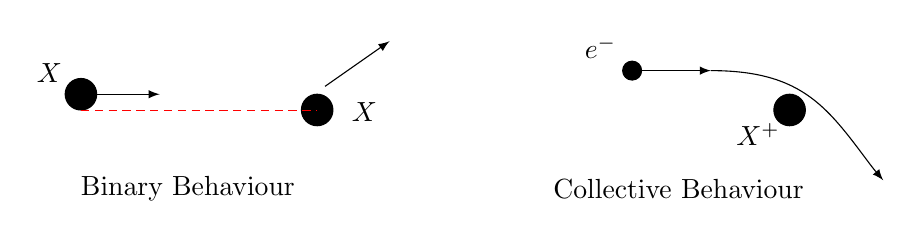
\begin{tikzpicture}
    \node [label={[shift={(0.6,-0.4)}] $X$}] (A) at (0,0) {};
    \node [label={[shift={(-0.4,-0.1)}] $X$}] (B) at (-3,0.20) {};
    \draw[black,fill=black] (B) circle (0.2);
    \draw[black,fill=black] (A) circle (0.2);
    \draw[-latex] (B) -- +(0:1); % Velocity arrow
    \draw[-latex] (0.1,0.3) -- +(35:1); % New velocity arrow
    \draw[red,line width=0.2pt, densely dashed] (-3,0.0) -- (0,0.0);
    \node[text width=3cm] at (-1.5,-1) {Binary Behaviour}; % Text node
    % End of binary collision
    % Start of collective collision
    \node [label={[shift={(-0.4,-0.7)}] $X^+$}] at (6,0) {};
    \node [label={[shift={(-0.4,-0.1)}] $e^-$}] at (4,0.5) {};
    \draw[black,fill=black] (4,0.5) circle (0.12);
    \draw[black,fill=black] ([shift=({6,0})]A) circle (0.2);
    \draw[-latex] (4,0.5) -- +(0:1); % Velocity arrow
    \draw[-latex] (7.06,-0.74) -- +(-50:0.2); % New velocity arrow
    \draw (5,0.5) .. controls (6.2,0.5) and (6.5,-0.0) .. (7.06,-0.74);
    \node[text width=4cm] at (5,-1) {Collective Behaviour}; % Text node
\end{tikzpicture}
  \end{figure}

  \footnotetext{The generated electromagnetic fields are regarded as properties of the plasma.}
  
\end{frame}
\begin{frame}{\collectivebehaviour}
  Indside such a medium, diverse collective phenomena can occur.

  This allows for electron acceleration in laser--driven plasma wake--fields.
\end{frame}
\subsection{The Spectrum of Hydrogen}
\newcommand{\hydrogenspecrum}{The Spectrum of Hydrogen}
\begin{frame}{\hydrogenspecrum}
%An electron making a transition between two energy levels emits a photon.

Hydrogen spectrum is divided into series, determined by the transitions to the final state.
\begin{itemize}
    \item $n_i=3 \to n_f=2$, \SI{656.23}{\nm} --- H\textsubscript{$\alpha$}
    \item $n_i=4 \to n_f=2$, \SI{486.13}{\nm} --- H\textsubscript{$\beta$}
\end{itemize}
\begin{figure}
  %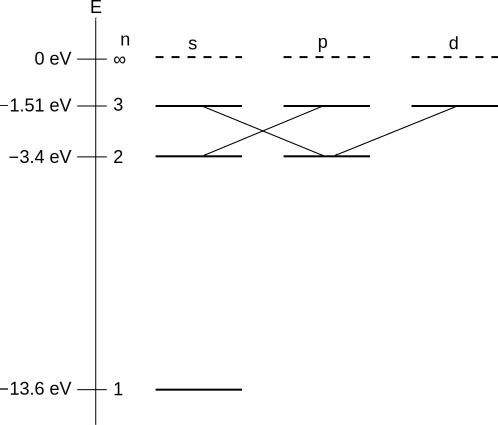
\includegraphics[width=100px]{figures/halphagrotrian.png}
    \def\svgwidth{0.48\textwidth}
    \input{figures/halphagrotrian.pdf_tex}
\end{figure}
Both H\textsubscript{$\alpha$} and H\textsubscript{$\beta$} are in the visible spectrum, and so are easy to observe.

Other series are Lyman ($n_f=1$) and Paschen ($n_f=3$).
\end{frame}
\begin{frame}{\hydrogenspecrum}
Spectroscopy study of such emission can give information about the physical conditions in the plasma, such as density and temperature.

Advantage: No probes --- no interferance in any way with the plasma.

Disadvantage: Radiation is collected only along the line of sight in the direction of observation.
\end{frame}
\begin{frame}{The emitted radiation process depends on:}
  The probability that 
 \begin{enumerate}
   \item there is an electron in the upper level of the transition,
   \item the electron transition is significant,
   \item the emitted photon escapes from the volume of the plasma without being absorbed.
 \end{enumerate} 
 We neglect process (3) and use the approximation of \emph{Optically thin plasma}.

 Values of the transition probabily $A_{i\to j}$ for process (2) are tabulated\footnote[frame]{See \url{https://physics.nist.gov/PhysRefData/ASD/lines_form.html} for example.}.
\end{frame}

\begin{frame}{Optical Depth}{Optically thin plasma}
  The optical depth $\tau$ (dimensionless) is a measure of the opacity of the medium:
  \begin{equation*}
    \tau=-\kappa z
  \end{equation*}
  $\kappa$ --- the linear absorption coefficient (\si{\per\cm}).

  $I_\text{out}$ and $I_\text{in}$ are related by
  \begin{equation*}
    I_\text{out} = I_\text{in}\mathrm{e}^{-\tau} %\tag{(Simplest)radiative transfer equation}
  \end{equation*}
\begin{columns}
  \column{0.4\textwidth}
      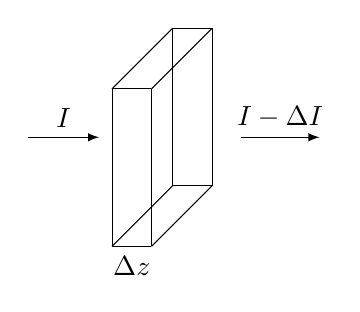
\begin{tikzpicture}
\draw(-0.25,1,1) -- (0.25,1,1);
\draw(-0.25,1,1) -- (-0.25,1,-1);
\draw(-0.25,1,1) -- (-0.25,-1,1);
\draw(0.25,1,1) -- (0.25,1,-1);
\draw(0.25,1,1) -- (0.25,-1,1);
\draw(0.25,1,-1) -- (-0.25,1,-1);
\draw(0.25,1,-1) -- (0.25,-1,-1);
\draw(-0.25,1,-1) -- (-0.25,-1,-1);
\draw(-0.25,-1,1) -- node [midway, below] {$\Delta z$} (0.25,-1,1);
\draw(0.25,-1,-1) -- (0.25,-1,1);
\draw(0.25,-1,-1) -- (-0.25,-1,-1);
\draw(-0.25,-1,-1) -- (-0.25,-1,1);
\draw[-latex] (-1.7,0,0) -- node [midway, above] {$I$} (-0.8,0,0);
\draw[-latex] (1,0,0) --  node [midway, above] {$I-\Delta I$} (2,0,0) ;


\end{tikzpicture}

    \column{0.6\textwidth}
  \begin{center}
  \begin{tabular}{ c c c }
    $\tau<1$ & $\longrightarrow$ & optically thin medium\\ 
    $\tau>1$ & $\longrightarrow$ & optically thick medium
  \end{tabular}
  \end{center}
\end{columns}
\end{frame}
\newcommand{\lte}{Local Thermodynamic Equilibrium(LTE)}
\begin{frame}{\lte}
  In an isolated, closed system where the radiation and matter have reached equilibrium (black body cavity) the distribution of the kinetic motions, level populations and radiation fields are described by well-defined function of a single parameter ---

  The system temperature.

  This situation is called \emph{complete thermodynamic equilibrium}.
\end{frame}
\begin{frame}{\lte}
  \begin{center}
\resizebox{\textwidth}{!}{%
  \begin{tabular}{ c | c}
  Radiation field  & $\rho(\nu)=\frac{8\pi}{c^{3}}\frac{\nu^{3}}{\mathrm{e}^{\frac{h\nu}{k_{B}T}}-1}$ \\ \hline
  Ionisation degree  & $\frac{N_2}{N_1}=\frac{g_2}{g_1}\mathrm{e}^{-\frac{E_2-E_1}{k_BT}}$ \\ \hline %Eq 6.68 from Ryden and eq II.4 from Verdeyen
  Populations ratio of bound quantum states  & $f\left(v\right)=4\pi\left(\frac{m}{2\pi k_{B}T}\right)^{3/2}v^{2}\mathrm{e}^{-\frac{1}{2}\frac{mv^{2}}{k_{B}T}}$ % eq 2.2.4 from Moshe Elitzur.
  % Important : What is then equation 5.69 in Ryden??? See also Tallents 12.7
\end{tabular}
}
\end{center}
Each temperature would be different from each other, and become the same only for a system in thermodynamic equilibrium --- a black body cavity.

Those equilibrium populations are achieved because collisional process dominate the radiative processes.
\end{frame}
\begin{frame}{Collisional Processes}{And their inverses}
  \begin{center}
\resizebox{\textwidth}{!}{%
  \begin{tabular}{ c | c | c }
  Ionisation  & $ \left(\ \right)^{-1} \rightarrow$ & Recombination \\
  \hline
  Excitation  &  $\overset{\left(\:\right)^{-1}}{\longleftrightarrow}$ & De--excitation \\
  \hline
\end{tabular}
}
\end{center}
Inverse collisional processes have a \emph{detailed balance} relationship to each other.
% From Tallents, between equations 12.2 and 12.3:
In equilibrium, the principle of detailed balance requires these inverse processes to occur at equal rates.

\end{frame}
\begin{frame}{Detailed Balance Implications}
Thus, knowing the rate coefficient (cross section, for example) for one process, we can compute its inverse rate coefficient.

But those collisional--rate coefficients are simply atomic parameters\footnotemark, and so are independent of the state of the plasma, and apply also to plasmas not in equilibrium.

If no other process occur (apart from the detailed balance process) the populations have the equilibrium values for the particular density and temperature of the plasma.
\footnotetext{NIST.gov}
\end{frame}
\begin{frame}{Line Broadening}
A perfectly sharp energy line is impossible, and thus there is a distribution of transitions from states near $E_2$ to $E_1$.
\end{frame}
\subsection{Classification of Radiation Transition}
\begin{frame}{Classification of Radiation Transition}
  \begin{columns}%[t]
  \begin{column}{0.6\textwidth}
  \begin{figure}
    \includegraphics[width=\textwidth]{figures/Deuterium_lamp_1.png} 
    \caption{Spectrum of light emitted by a deuterium lamp}
  \end{figure}
  \end{column}  
  \begin{column}{0.4\textwidth}
  The contributions to the spectrum emitted by a plasma are classified according to their type:
  \begin{itemize}
    \item continuum, or
    \item line radiation
  \end{itemize}
  \end{column}
  \end{columns}
\end{frame}
\begin{frame}{Radiation Transition}
  \begin{columns}%[t]
  \begin{column}{0.6\textwidth}
  \begin{enumerate}
    \item Free--free transition. Both initial and final electron states are in continuum. Usually infared.
    \item Free--bound transition. Electron transition between a free state in continuum and a bound state in atom.
    \item Bound--bound transition. Electron transition between discrete atomic levels, results in emission (and absorption) of spectral lines.
  \end{enumerate}
  \end{column}
  \begin{column}{0.4\textwidth}
  \includegraphics[width=\textwidth]{figures/radiationTransition.tikz}
  \end{column}
  \end{columns}
\end{frame}
\begin{frame}
  All transitions emit spectral lines that have finite width.
  
  The observed line shape function $f(\lambda)$ and its width $\Delta \lambda_{1/2}$ depend on the temperature and pressure of the emitting plasma.
\begin{figure}
\includegraphics[width=0.7\textwidth,height=0.3\textwidth]{figures/theory/lineshape.tikz}
\end{figure}
The dominant cause of line Broadening in plasma is the inter--atomic Stark effect.
\end{frame}
\begin{frame}{Stark effect}
  Plasma is a charged medium.

  When the density of charged particles is sufficiently large, their electric micro--fields perturb the atomic energy levels.
  \begin{figure}
      \includegraphics[width=0.7\textwidth]{figures/stark_effect_1.png}
  \end{figure}
  The splitting of states by an electric field is called the \emph{Stark effect}.

  Measurement of Stark half-widths --- reliable and convinient method for the determination of electron densities.
  \end{frame}
  \begin{frame}{Stark effect}
    Since the distance of the perturber is continuously changing, the line shift also changes accordingly giving rise to what is called the Stark Broadening.
    \begin{figure}
    \includegraphics[width=0.5\textwidth]{figures/starkBroadening.tikz}
    \end{figure}
  \end{frame}
  \begin{frame}{Stark effect}
    The line shape for the Stark broadening takes that of a Lorentzian:
    \begin{equation*}
      I\left( \lambda \right)=\frac{A^2}{4\left( \left(\lambda-\lambda_0\right)^2+\Delta \lambda_{1/2}^2\right)}
    \end{equation*}
    \begin{figure}
\includegraphics[width=\textwidth,height=0.5\textwidth]{figures/lorentzian_lineshape.tikz}
    \end{figure}
    \resizebox{\textwidth}{!}{%
  \begin{tabular}{ c c }
    The relation between density and the line width is tabulated: & $n_e=\left( \frac{\Delta\lambda_{1/2}}{\gamma\left(n_e,T_e\right)}\right)^{3/2}.$
    \\
    Weak dependence on temperature. In our experinemt we work with & $n_e\left[\SI{e18}{\per\cubic\cm}\right]=\left( \frac{\Delta\lambda_{1/2}\left[\si{\nm}\right]}{5.4}\right)^{3/2}.$
  \end{tabular}
    }
\end{frame}
\begin{frame}{Stark effect}
  \begin{columns}
    \column{0.4\textwidth}
    \begin{figure}
      \includegraphics[width=\textwidth]{figures/lorentzian_lineshape.tikz}
    \end{figure}
    \column{0.6\textwidth}
    Relation between $N_e$ and $\Delta \lambda_{1/2}$ is tabulated: $$N_e=\left( \frac{\Delta\lambda_{1/2}}{\gamma\left(n_e,T_e\right)}\right)^{3/2}.$$
    \\
    Weak dependence on temperature, in our experiment: $$N_e\left[\SI{e18}{\per\cubic\cm}\right]=\left( \frac{\Delta\lambda_{1/2}\left[\si{\nm}\right]}{5.4}\right)^{3/2}.$$
  \end{columns}
  \end{frame}
  \subsection{Plsama acceleration, laser wake--field acceleration}
  \begin{frame}{LWFA}
  Originally proposed by Toshiki Tajima and John Dawson in 1979,
  
  on purpose for experiments on nuclear physics and the structure of matter.
  \begin{figure}
    \includegraphics[height=0.7\textheight]{figures/PhysRevLett.43.267.pdf}
  \end{figure}
  \end{frame}
  \begin{frame}{LWFA}{Limitations}
    Two limitations preventing well--defined particle beams:
    \begin{description}
      \item[Defocusing of the laser radiation] Transverse spreading of the wake--driving laser when propagating within the plasma. Withput optical guiding, the wake would propagate over a distance of the order of the Rayleigh length.
      \item[Electron dephasing length] The distance over which an ultra relativistiv electron outruns the wakefield and no longer gains energy.
    \end{description}
  \end{frame}
  \begin{frame}{A brief review of Gaussian beams}
    The divergence of a laser beam is usually neglected.

    This is not the case in a plasma accleration.
    
    Acceleration is achieved only when the laser beam is focused to a tiny spot of a few tens of microns in diameter.

    \begin{center}
      plot of a beam through a lens with numbers, Rayleigh length of about 0.4 mm.
    \end{center}
    We need to extend this length.

    Solution: Use a waveguide.
  \end{frame}
  \begin{frame}{Waveguides}{Basic concept}
  \begin{figure}
     \includegraphics[width=\textwidth]{figures/fiber.tikz}
   \end{figure}
   Total internal reflection resulting from axially--peaked refraction index.

   A transparent core in which light is confined and a cladding with a smaller refractive index.
  \end{frame}
  \begin{frame}{Solution: Construct a plasma waveguide}
    Making a tightly focused laser pulse propagate over many tens of Rayleigh lengths without divergence ---

    construct a preformed plasma channel with radially increasing density.

    Contrary to optical fibers, plasma waveguides
    \begin{enumerate}
      \item form dynamically
      \item continuous radial decrease of $\tilde n$
      \item results from the increase of plasma density
    \end{enumerate}
  \end{frame}
  \begin{frame}{Preformed plasma channel}
  The dispersion relation for an electromagnetic wave propagating in a plasma is
  \begin{equation}
    \omega^2=\omega_p^2+c^2k^2
  \end{equation}
  The index of refraction $\tilde n$ is
  \begin{equation}
    \tilde{n}=\frac{c k}{\omega}=\sqrt{1-\frac{\omega_p^2}{\omega^2}}\approx1-\frac{\omega_p^2}{2\omega^2}=1-\frac{N_e}{2N_\text{cr}}
  \end{equation}
  where
    \begin{equation}
        N_\text{cr}=\frac{\omega_L^2\varepsilon_0 m_e}{e^2}
    \end{equation}
    is the critical plasma density.

    The plasma is called \textit{underdense} for $N_e < N_\text{cr}$, with $N_\text{cr}\sim\SI{1.7e21}{\per\cubic\cm}$ for an \SI{800}{\nm} laser.
\end{frame}
  \begin{frame}{Preformed plasma channel}{continued}
    If the refractive peaks on the axis of a plasm channel, because of lower density, then we have a waveguide ---

    focused laser radiation propagates along the channel.

    Ideally, the radial density profile (RDP) is parabolic:
     \begin{equation*}
      N_e(r)=N_e(0)+\Delta N_e\left( \frac{r}{r_\text{ch}}\right)^2
    \end{equation*}
    \begin{center}
      figure of rdp
    \end{center}
  \end{frame}
  \begin{frame}{Mathcing conditions}
    The matched radius of the guided beam is \cite{}
   \begin{equation*}
     w_m=\left( \frac{r_\text{ch}^2}{\pi r_e \Delta N_e}\right)^{1/4}
   \end{equation*}
   $\Delta N_\text{min}$ should be about \SI{2e16}{\per \cubic \cm}.
  \end{frame}
  \begin{frame}{Methods for creating a plasma channel}
    Electrical discharge in an initially evacuated capillary.
    \begin{description}
      \item[Ablated capillary] Ablating and subsequently ionizing the wall material. Ablation leads to loss of wall material, and therefore a shorter capillary lifetime.
      \item[Gas--filled capillary] Pre--filled with gas, such as hydrogen, at a pressure of several bars. %Ionization of the gas -> longer device lifetime.
    \end{description}
    \begin{tabular}{cc}
    \includegraphics[width=0.5\textwidth]{figures/theory/ablated.png} & \includegraphics[width=0.5\textwidth]{figures/theory/gasfilled.png}
    \end{tabular}
    %% Mathematica code to render these stl files:
    % Import["figures\\5-\ 500-S.STL", "Graphics3D", ImageSize -> imageSize, ViewAngle -> All, Lighting -> Automatic, ViewVertical -> {0, 1, 0}, BaseStyle -> RGBColor[0.7, 0.8, 0.86], ViewPoint -> {1.5, 0.9, 2.3}]
  \end{frame}
  %\begin{frame}{Why the channel forms}
    %But why the plasma channel forms?

    %What causes the density to be lower on the axis then away from it?
    %\begin{figure}
      %\includegraphics[width=0.4\textwidth]{figures/radial_density.pdf}
    %\end{figure}
  %\end{frame}
  \begin{frame}{Why the channel forms}{Explanation}
    Initial pressure variations are being wiped out rapidly because they travel at the plasma speed of sound, $$v_s=\sqrt{k_B T_e/M}\sim \SI{e6}{\cm\per\s}$$ for $T_e\sim\SI{1}{\electronvolt}.$ I.e., a characteristic time scale for a perturbation to propagate would be
    $$\Delta T=\frac{L}{v_s}=\SI{25}{\ns}.$$
    Under assumption of the ideal gas equation--of--state, $P=N_e k_B T$, this implies a uniform pressure.
  \end{frame}
  \begin{frame}{Why the channel forms}{Explanation, continued}
      Heat transfer (or heat conduction) from the electrons to the wall cools the electrons there, causing the current density near the wall to decrease. 
     \begin{figure}
       \includegraphics[width=0.4\textwidth]{figures/theory/why channel forms.png}
     \end{figure}
      The heating of the plasma is mostly Ohmic, and is balanced mainly by thermal conduction at the capillary wall. This results in current density increase near capillary axis, and, consequently, a higher temperature there.
  \end{frame}
  \begin{frame}{Multi--stage acceleration scheme}
    As stated previously, there is also the dephasing length limitation:
    
    trapped electrons outrun or dephase the acclerating phase of the wakefield.
    
    The current paradigm is a multi--stage accelerator, composed of multiple stages.
    
    Optimization by matching the dephasing length to the depletion length of the laser pulse.

    \begin{figure}
      \includegraphics[width=0.6\textwidth]{figures/coupling_scheme.pdf}
    \end{figure}
  \end{frame}
  \section{Goals}
  \begin{frame}{Thesis Goals}
    \begin{enumerate}
      \item Study of discharge evolution, low jitter of discharge ignition.
      \item Demonstration of optical guiding.
      \item Spectroscopy analysis, utilizing Stark broadening.
      \item Development of multi stage capillary --- fish bone approach.
    \end{enumerate}
  \end{frame}
  \begin{frame}{Experiment Scheme}
    \begin{figure}
      \includegraphics[width=\textwidth]{figures/methods/Laser-based ignition scheme.png}
    \end{figure}
    Capillary inside a vacuum chamber, maintained at \SI{e-4}{\torr}
  \end{frame}
  \begin{frame}{Experiment Scheme}{continued}
    \begin{figure}
      \includegraphics[width=\textwidth]{figures/methods/system_picture.jpg}
    \end{figure}
  \end{frame}
  \begin{frame}{Experimental Results}{Low Jitter}
    A typical plasma discharge. Damped oscillatory current profile.
    \begin{figure}
      \includegraphics[]{figures/results/typical.png}
    \end{figure}
    Requirement for a ready--to--use guiding media --- low jitter.
  \end{frame}
  \begin{frame}{Experimental Results}{Low Jitter}
    12 cosecutive capillary discharges. Demonstrating low ignition jitter.
    \begin{figure}
      \includegraphics[width=0.4\textwidth]{figures/results/low_jitter.png}
    \end{figure}
    $$\tau_\text{jitter}\approx 1\pm 0.36 \si{\ns}$$
  \end{frame}
  \begin{frame}{Experimental Results}{Low Jitter}
    Without the igniting laser pulse - much less stable regime.
    \begin{figure}
      \includegraphics[width=0.4\textwidth]{figures/results/high_jitter.png}
    \end{figure}
    $$\text{jitter}\approx \SI{80}{\us}$$
  \end{frame}
  \begin{frame}{Experimental Results}{Low Jitter}
    These results conributed to two publications:
    Thses results apply to two types of plasmas created in capillaries:
    \begin{enumerate}
      \item For PLWA: Biagioni Angelo and Behar Ehud et al. \emph{"Gas filled capillary dis-charge stabilization for plasma based accelerators by means of alaser pulse"}. In: \emph{Optical Letters.} Accepted for publication.
      \item For LWFA: Raz Yoav and Behar Ehud et al. \emph{Low jitter parabolic profile low density plasma channel in 3D printed gas filled capillary}. In: Plasma research express. Accepted for publication.
    \end{enumerate}
    Different plasma characteristics, but need for low jitter system is common.
  \end{frame}
  \begin{frame}{Duration of the parabolic density profile}{System setup}
    System setup as before, but now adding an oscillator laser.
    \begin{figure}
     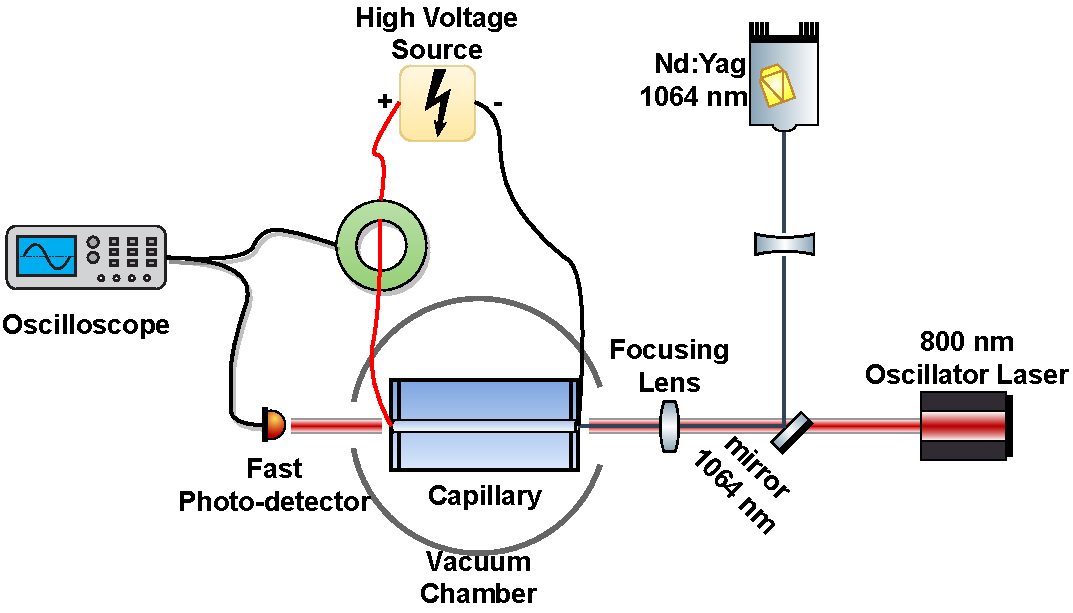
\includegraphics[width=\textwidth]{figures/results/oscillator/oscillator_system_setup.png} 
    \end{figure}
    Beam aligned throught the capillary, to a fast photo--diode.
  \end{frame}
  \begin{frame}{Duration of the parabolic density profile}{System setup}
    Oscillator laser, \SI{800}{\nm}, pulses at a \SI{84}{\MHz} rate.
    \begin{figure}
      \includegraphics[width=0.7\textwidth]{figures/results/oscillator/single.PNG}
    \end{figure}
  \end{frame}
  \begin{frame}{Duration of the parabolic density profile}
    Upon plasma discharge, we look for an increase in the detected amplitude --- optical guiding.
    \begin{equation*}
      \text{transmission ratio} = \frac{A_{t<0}}{A_\text{max}}
    \end{equation*}
    \begin{figure}
      \includegraphics[width=\textwidth]{figures/results/oscillator/results01.PNG}
    \end{figure}
  \end{frame}
  \begin{frame}
    Another frame witht results02.png
  \end{frame}
  \begin{frame}{Duration of the parabolic density profile}{Explanation}
    If an inverted radial density profile is created, a plasma lens forms and the radiation is focused and trapped by the plasma.
    \begin{figure}
      \includegraphics[width=0.7\textwidth]{figures/results/oscillator/chen4_31.png}
    \end{figure}
    Note: The radiation is blocked in the later stage of the discharge, until the plasma is diffused.
    \begin{figure}
      \includegraphics[width=0.4\textwidth]{figures/results/oscillator/not_opaque.PNG}
    \end{figure}
  \end{frame}
  \begin{frame}{Duration of the parabolic density profile}{Explanation}
    Correlation between applied voltage and the transmission ratio:
    \begin{figure}
      \includegraphics[width=0.4\textwidth]{figures/results/oscillator/voltage vs guiding.png}
    \end{figure}
    Duration of the plasma channel:
    \begin{equation*}
      \Delta t_\text{channel}=50 -100\ \si{\ns}.
    \end{equation*}
  \end{frame}
  \begin{frame}{Spectroscopy measurements}
    Quantitative estimation of the depth of the plasma channel and the plasma density.

    A measurement with a spectrometer and a fast camera.
    \begin{columns}
      \column{0.5\textwidth}
          \includegraphics[width=0.5\textwidth]{figures/results/spectro/spectrometer.png}
      \column{0.5\textwidth}
      drawing of the ccd output?
    \end{columns}
    Both radial and longitudinal density profile.
  \end{frame}
  \begin{frame}{Spectroscopy measurements}{System setup}
Radial density profile
\begin{figure}
  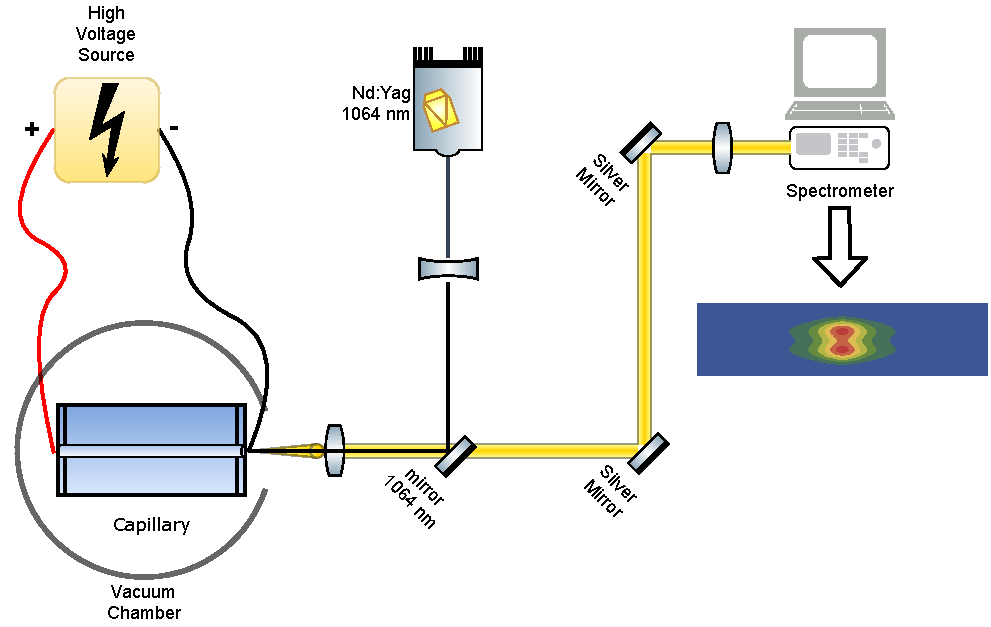
\includegraphics[width=0.8\textwidth]{figures/results/spectro/radial_system.png}
\end{figure}
Imaging system --- $\times 5$ magnification.

CCD camera $\SI{40}{\ns}$ gate--on time. 

Width of the spectrometer slit --- \SI{150}{\um}.
  \end{frame}
  \begin{frame}{Spectroscopy measurements}{Analysis}
    \begin{figure}
      \includegraphics[width=0.8\textwidth]{figures/results/spectro/spectra_analysis.png}
    \end{figure}
    pixel size = $\SI{26}{\um} \times \SI{26}{\um}$
  \end{frame}
  \begin{frame}{Spectroscopy measurements}
    Fit a Lorentzian to each row of the data.
    \begin{figure}
      \includegraphics[width=0.8\textwidth]{figures/results/spectro/sample-lorentzian.png}
    \end{figure}
    Stark Broadening on the order of \SI{3}{\nm}.
  \end{frame}
  \begin{frame}{Spectroscopy measurements}{Radial density profile}
    Density minimum on the axis of the capillary.
    \begin{equation*}
      \Delta N_e \sim \SI{0.4e18}{\per \cubic \cm}
    \end{equation*}
    with
    \begin{equation*}
      r_\text{ch}\approx \SI{50}{\um} \text{ and } N_e\left(0\right)\approx \SI{0.4e18}{\per\cubic\cm}.
    \end{equation*}
    \begin{figure}
      \includegraphics[width=0.8\textwidth]{figures/results/spectro/parabolic_profile.png}
    \end{figure}
    These conditions provide an optimal plasma channel that can be used for guiding an intense laser pulse for LWFA accelerators.
  \end{frame}
  \begin{frame}{Longitudinal density profile}
    Verify longitudinal homogeneity of the plasma density.
    \begin{figure}
      \includegraphics[width=0.8\textwidth]{figures/results/spectro/longitudinal_system.png}
    \end{figure}
    The entire capillary length was imaged.
    CCD camera \SI{1}{\us} gate--on time.
  \end{frame}
  \begin{frame}{Longitudinal density profile}{Results}
    Measurement result: Mean plasma density $\bar{N}_e$ of
    \begin{equation*}
        \bar{N}_e \sim \SI{3e17}{\per\cubic\cm}.
    \end{equation*}
    \begin{figure}
      \includegraphics[width=0.9\textwidth]{figures/results/spectro/longitudinal_profile.png}
    \end{figure}
  \end{frame}
  \begin{frame}{Two stage capillary}
    As said in the introduction, a "fish--bone" capillary may overcome the dephasing length limitation.
     \begin{figure}
     \includegraphics[width=0.2\textwidth]{figures/coupling_scheme.pdf}
     \end{figure}
     \begin{figure}
     \includegraphics[width=0.8\textwidth]{figures/results/2stageCapillary/doublecapillary_cad.png}
     \end{figure}
     A 2 stage, Y--shape capillary.
  \end{frame}
  \begin{frame}{Two stage capillary}
    Split the oscillator pulse--train to two beams, one for each capillary channel.
    
    Introduce a delay line to distinguish between each beam.
    \begin{figure}
      \includegraphics[width=0.6\textwidth]{figures/results/2stageCapillary/double.png}
    \end{figure}
  \end{frame}
  \begin{frame}{Two stage capillary}{System setup}
    \begin{figure}
      \includegraphics[width=0.6\textwidth]{figures/results/2stageCapillary/double.png}
    \end{figure}
    \begin{figure}
      \includegraphics[width=0.3\textwidth]{figures/results/2stageCapillary/line-of-sight.png}
    \end{figure}
    No line--of--sight for the curved capillary. Relying on refractions from the plastic walls.
  \end{frame}
  \begin{frame}{Results}
    First check, jitter controlled system.
    \begin{figure}
      \includegraphics[width=0.8\textwidth]{figures/results/2stageCapillary/low_jitter_curved_capillary.png}
    \end{figure}
    Jitter--controlled ignition when the Nd:Yag pulse is delivered to the \textbf{positive} electrode.

    Jitter on the same scale as in the straight capillary - $\tau_\text{jitter}\approx 1\pm \SI{0.5}{\ns}$.
  \end{frame}
  \begin{frame}{Results}
    \begin{figure}
      \includegraphics[width=0.8\textwidth]{figures/results/2stageCapillary/curved-pulsetrain-merged.png}
    \end{figure}
    \begin{columns}
      \column{0.8\textwidth}
        Note the "bump" of the signal recorded by the photo--diode.

        To minimize this, use a screen to block as much unwanted light.
    \column{0.2\textwidth}
      \includegraphics[width=1\textwidth]{figures/results/2stageCapillary/opaquescreen.png}
    \end{columns}
  \end{frame}
\end{document}